\begin{frame}{Otra diapositiva} %%Otra forma (más corta) de poner el título a la diapositiva
Texto adicional. No tiene un propósito en particular más que ocupar algo de espacio.
Texto adicional. No tiene un propósito en particular más que ocupar algo de espacio.
Texto adicional. No tiene un propósito en particular más que ocupar algo de espacio.
Texto adicional. No tiene un propósito en particular más que ocupar algo de espacio.
\( \sum_0^{\infty} a_i \) 
Texto adicional. No tiene un propósito en particular más que ocupar algo de espacio.
\end{frame}

\section{Sección de ejemplo 2} %%Otra sección
\begin{frame}
    \frametitle{Un teorema}
    
    \begin{teorema} %%Uso del "environment" definido al inicio del documento.
        Los números primos son infinitos
    \end{teorema}

    Y algo de texto
    
    \centering 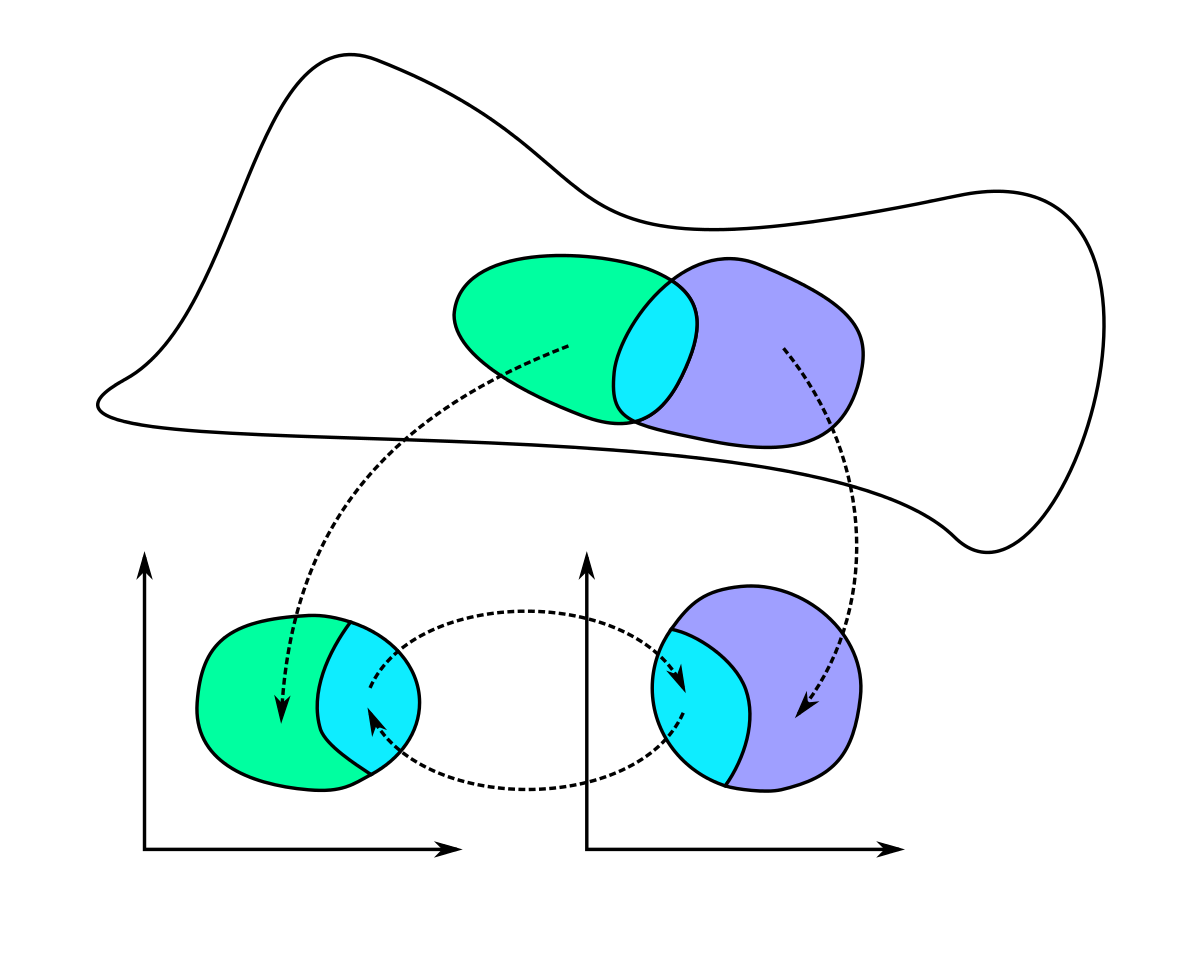
\includegraphics[width=0.45 \paperwidth]{images/Manifold1.png}
\end{frame}

\section{Teorema con referencia}
\begin{frame}{Ejemplo}
\framesubtitle{Incluye referencia}
    \begin{teorema}[Teorema de Stokes]
        Sea $M$ una variedad compacta orientada con frontera, $\omega$ una $k-1$-forma sobre $M$, entonces $$\int_{M} d\omega = \int_{\partial M} \omega$$
    \end{teorema}

    la prueba se puede revisar en: \cite{spivak2018calculus}
\end{frame}

\section{Referencias}
\begin{frame}{Referencias}
    %posibles estilos para bibliografía: unsrt , siam , plain , ieeetr , alpha , acm , abbrv
    \bibliographystyle{apalike}
  \bibliography{references}
\end{frame}


\begin{frame}{Gracias}
    
\end{frame}

\end{document}
